\documentclass[british,fleqn]{article}
\usepackage{default}

\title{%
  \textsf{IN3160V22 --- Oblig 9}\\%
  \textsf{Pipelining and bits in arithmetic calculations}%
}
\author{%
  \sffamily Martin Mihle Nygaard
  \sffamily\href{mailto:martimn@ifi.uio.no}{<martimn@ifi.uio.no>}%
}

\begin{document}
\maketitle

\titlelabel{\thetitle.\quad}
\titleformat{\section}[hang]
  {\bfseries}
  {\thesection.}
  {1em}
  {\normalfont}
%\titlespacing{\section}{0pt}{3em}{1em}[0pt]
\renewcommand{\thesubsection}{\alph{subsection}}
\titleformat{\subsection}[hang]
  {\bfseries}
  {(\thesubsection)}
  {1em}
  {\normalfont}
\titlespacing{\subsection}{2em}{.5\baselineskip}{.5\baselineskip}[0pt]
\lstMakeShortInline[basicstyle=\ttfamily]`

\section[Task 1]{%
  We have two numbers $a$ and $b$ which is 16 bits each. How many bits
  is the result of the sum of these two numbers (i.e. $a + b$)?%
}

Let both $a$ and $b$ be $2^{16}$, the highest value a 16-bit number can
hold.\footnote{Or possibly $2^{16}-1$ if you exclude 0, but it doesn't really
matter for the final results, just makes the calculations messier.} Then we
have:
\begin{equation*}
  \log_2\del{a + b} = \log_2\del{2\times{2^{16}}} = \log_2\del{2^{17}} = 17.
\end{equation*}

\section[Task 2]{%
  How many bits is the result of mulitiplying these two 16 bits numbers
  (i.e. $a \cdot b$)?%
}

With $a$ and $b$ as before, we have 
\begin{equation*}
  \log_2\del{a \cdot b}              =
  \log_2\del{{2^{16}}\times{2^{16}}} =
  \log_2\del{2^{32}}                 = 32.
\end{equation*}

\section[Task 3]{%
  We now have four numbers: $a$, $b$, $c$, and  $d$ who are 16 bits each. How
  many bits is the result of adding all these numbers $a + b + c + d$?%
}

Same logic:
\begin{equation*}
  \log_2\del{a + b + c + d}   =
  \log_2\del{4\times{2^{16}}} =
  \log_2\del{2^{18}}          = 18.
\end{equation*}

\section[Task 4]{%
  We now have a additional number $e$ which is 16 bits. How many bits is the
  result of $\del{a+b+c+d} \times e$?%
}

And finally, using the previous result: 
\begin{equation*}
  \log_2\del{\del{a + b + c + d}\times e} =
  18 + \log_2\del{2^{16}}                 =
  18 + 16                                 = 34.
\end{equation*}

\section[Task 5]{%
  Draw datapath diagrams for \lstinline{compute} and
  \lstinline{compute_pipelined}.%
}

\setlength{\leftmargini}{4em}%
\begin{itemize}
  \item[\bfseries(a)] See \autoref{fig:compute}.
    \begin{figure}
      %\centering
      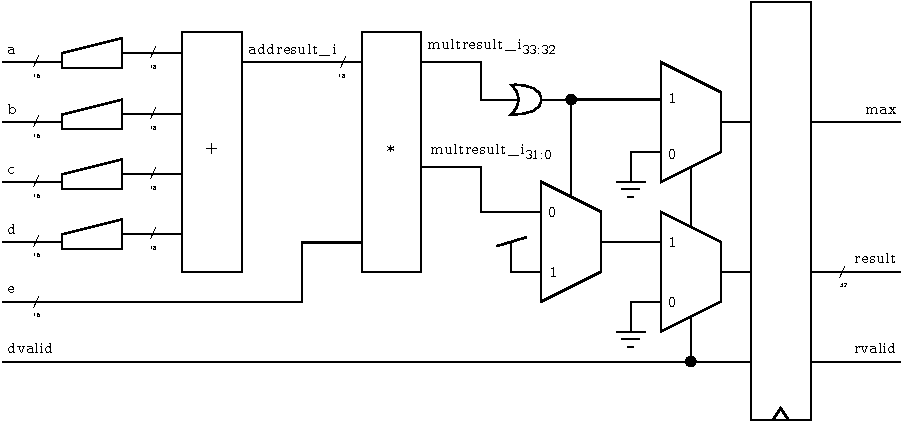
\includegraphics{compute.pdf}
      \caption{Datapath diagram for the \lstinline{compute} module. Reset
      functionality not included. I guess the add operation, \lstinline{+},
      should technically have been a tree of three two-input blocks instead,
      but I have abstracted this away for simplicity.}
      \label{fig:compute}
    \end{figure}
  \item[\bfseries(b)] See \autoref{fig:compute_pipelined}.
    \begin{figure}
      %\centering
      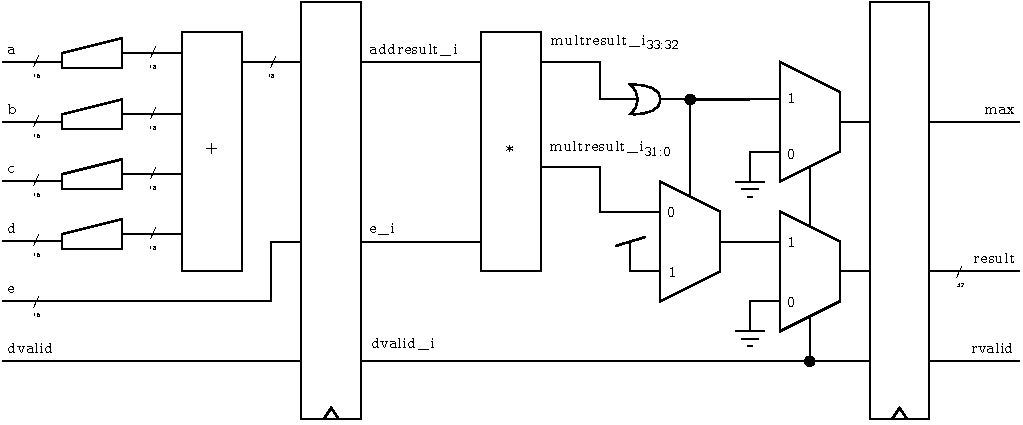
\includegraphics{compute_pipelined.pdf}
      \caption{Datapath diagram for the \lstinline{compute\_pipelined} module.
      Reset functionality not included.}
      \label{fig:compute_pipelined}
    \end{figure}
\end{itemize}

\section[Task 6]{%
  Implement the new module \lstinline{compute\_pipelined} in synthesizable
  \textsc{vhdl} based on the given compute \textsc{rtl} architecture. The given
  testbench \lstinline{tb_compute_pipelined} shall be used to ensure that the
  \lstinline{compute_pipelined} architecture works as required.%
}

The code for the module is attached as a separate file, but is also quoted in
\autoref{lst:compute_pipelined}. In my tests, it completed the attached
`tb_compute_pipelined.vhd` test bench without issue.

\lstinputlisting[
  language=VHDL,
  basicstyle=\tt\color{darkgray},
  numberstyle=\color{lightgray},
  keywordstyle=\color{black},
  float,
  label=lst:compute_pipelined,
  xleftmargin=0em,
  xrightmargin=0em,
  caption={%
    Source file \lstinline{compute_pipelined_rtl.vhd}. Modified from the
    included \lstinline{compute_rtl.vhd}. I've tried to put a comment on all my
    changes, but see \autoref{fig:compute_pipelined} for a more intuitive
    understanding of the new signals I've introduced.%
  }
]{../src/compute_pipelined_rtl.vhd}

\section[Task 7]{%
  How many registers/flip-flops are used in the module \lstinline{compute}?%
}

We need to store the `max`, `result` and `rvalid` signals between clock cycles.
These are the output signals. This is $1 + 32 + 1 = 34$ bits (I think).
\marginnote{\tt TODO: Check with Vivado's synthesis tool.}

\section[Task 8]{%
  How many registers/flip-flops are used in the module
  \lstinline{compute_pipeline}?%
}

We need to also store `dvalid_i`, `e_i` and `addresult_i` in addition the
same signals as in `compute`. This is $1 + 16 + 18 + \sbr{34} = 69$ bits.
\marginnote{\tt TODO: Check with Vivado's synthesis tool.}

\end{document}
